% F089｜勾股整数数组的构造规律｜05_traps.tex
% 继承上传模板的 LaTeX 环境；当前条目的内容独立编写。
\clearpage
\begin{trapbox}
\textbf{\textcolor{CTrap}{易错一：把生成的一组当成全部}}
\par\medskip
\begin{center}
% F089｜odd 原创简明教学示意图
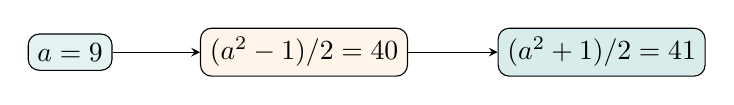
\begin{tikzpicture}[>=stealth,scale=.9]
\node[draw,fill=teal!10,rounded corners] (a) at (0,0){$a=9$};
\node[draw,fill=orange!8,rounded corners] (b) at (3.3,0){$(a^2-1)/2=40$};
\node[draw,fill=teal!15,rounded corners] (c) at (7.5,0){$(a^2+1)/2=41$};
\draw[->] (a)--(b);\draw[->] (b)--(c);
\end{tikzpicture}

\end{center}
\medskip
已知直角边为 $9$，奇数快捷式给出 $(9,40,41)$，但 $(9,12,15)$ 也成立。若题目问\textbf{所有组合}，必须用 F090 的因数配对法。
\end{trapbox}
\clearpage
\begin{trapbox}
\textbf{\textcolor{CTrap}{易错二：m和n随便取}}
\par\medskip
\begin{center}
% F089｜formula 原创简明教学示意图
\begin{tikzpicture}[>=stealth,scale=.9]
\node[draw,rounded corners,fill=teal!9] (a) at (0,0) {$m>n>0$};
\node[draw,rounded corners,fill=orange!10] (b) at (4.5,0) {$m^2-n^2,\ 2mn,\ m^2+n^2$};
\draw[->,thick] (a)--(b);
\node at (4.5,-1){\small 任取正整数 $m>n$，都会得到一组勾股数};
\end{tikzpicture}

\end{center}
\medskip
必须是正整数且 $m>n$；若 $m=n$，则 $m^2-n^2=0$，不再是正整数直角三角形。
\end{trapbox}
\clearpage
\begin{trapbox}
\textbf{\textcolor{CTrap}{易错三：所有构造结果都互质？}}
\par\medskip
\begin{center}
% F089｜triangle 原创简明教学示意图
\begin{tikzpicture}[>=stealth,scale=.9]
\coordinate (A) at (0,0);\coordinate (B) at (4,0);\coordinate (C) at (0,3);
\fill[teal!12] (A)--(B)--(C)--cycle;\draw[very thick,teal] (A)--(B)--(C)--cycle;
\draw (.3,0)--(.3,.3)--(0,.3);
\node[below] at (2,0){$4$};\node[left] at (0,1.5){$3$};\node[right] at (2,1.6){$5$};
\node[anchor=west] at (5,2.1){$3^2+4^2=5^2$};
\node[anchor=west] at (5,1.3){\small 直角边的平方和};
\node[anchor=west] at (5,.8){\small 等于斜边平方};
\end{tikzpicture}

\end{center}
\medskip
不一定。例如 $m=3,n=1$ 得到 $(8,6,10)$，三数可同时除以2。构造公式保证勾股关系，\textbf{不保证三边没有公因数}。
\end{trapbox}
